\documentclass[12pt]{article}
\usepackage[UTF8]{ctex}
\usepackage{pythonhighlight}
\usepackage{markdown}
\usepackage{listings}

\lstset{language=C++, %用于设置语言为bash
    keywordstyle=\color{purple}\bfseries, %设置关键词为蓝色,需要引xcolor宏包
    identifierstyle=\color{brown!80!black},
    basicstyle=\small, 
    commentstyle=\it\color[RGB]{100,100,100},%基本和注释的字体都使用默认的等宽,而非texlive调用的中文字体
    showstringspaces=false, %不显示中间的空格
    %frame=trBL,  %边框
    %frame=leftline,topline,rightline, bottomline,
    numbers=left,
    numberstyle=\it
}


% Language setting
% Replace `english' with e.g. `spanish' to change the document language
\usepackage[english]{babel}
\usepackage{float}
% Set page size and margins
% Replace `letterpaper' with `a4paper' for UK/EU standard size
\usepackage[letterpaper,top=2cm,bottom=2cm,left=3cm,right=3cm,marginparwidth=1.75cm]{geometry}

% Useful packages
\usepackage{amsmath}
\usepackage{graphicx}
\usepackage[colorlinks=true, allcolors=blue]{hyperref}

\title{Project2 Hard}


\begin{document}
\maketitle

\begin{abstract}
    Voting Tree
\end{abstract}

\section*{Chapter 1:Introduction}
Give all coordinate points of two polygons in clockwise direction,The graph with more coordinate points 
has a subgraph similar to the graph with fewer coordinate points,and the order in which the points of 
the subgraph appear must be cyclic monotonic,such as:if there are 5 points,the result such as (1,2,3,4,5),
(5,4,3,2,1),(3,4,5,1,2),(3,2,1,5,4) are all submitted,a simple example is as follows:
    \begin{figure}[H]
	\centering
	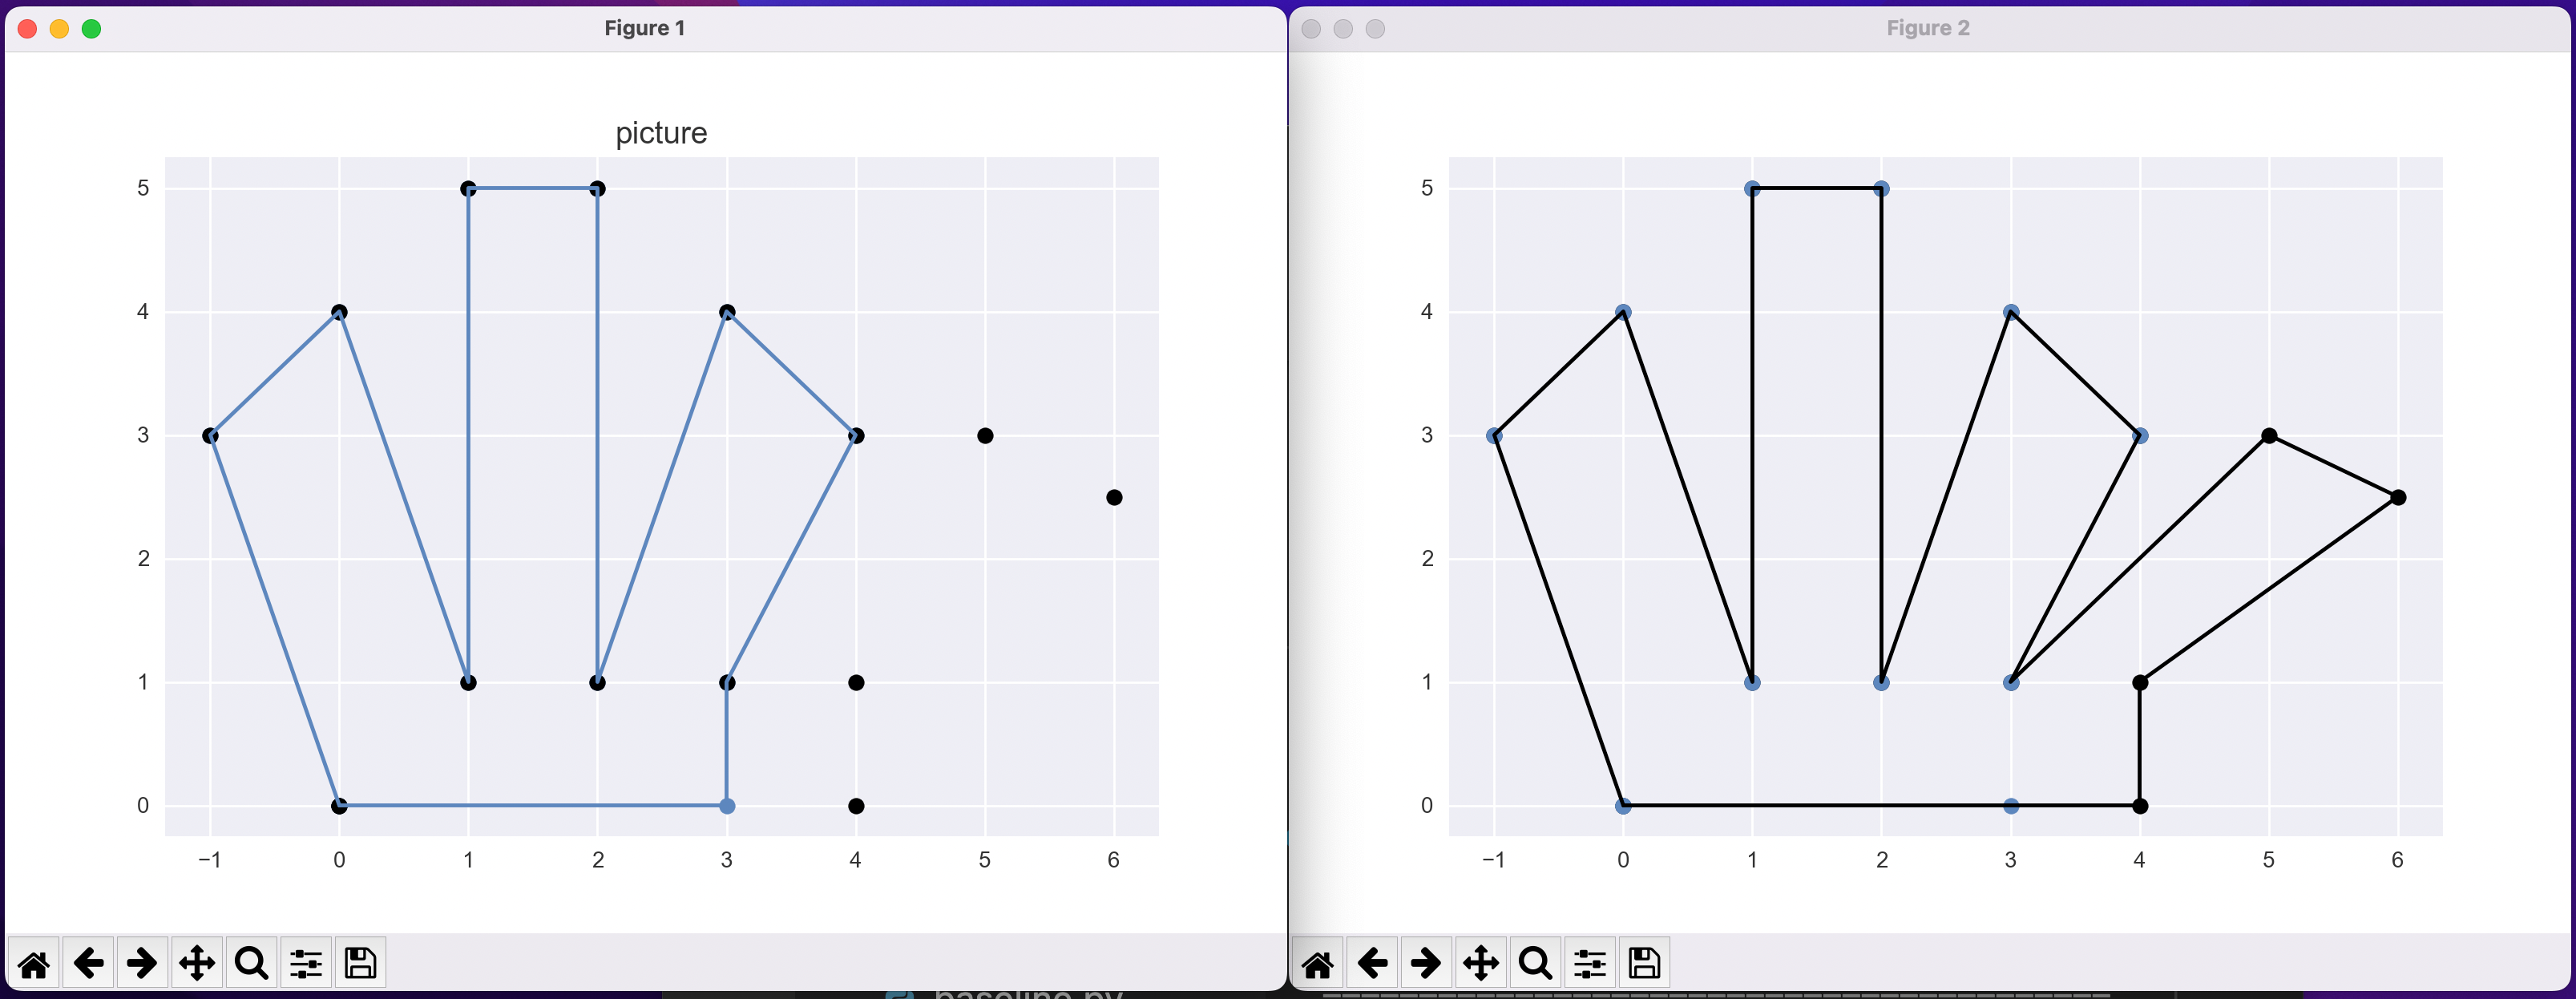
\includegraphics[width=0.9\textwidth]{1.png}
	\caption{\label{pr}Voting Tree Demo}
	\end{figure}
Your task is to find the best subgraph match like this.

In this project you should use the data structures including voting tree and arrays,The basic idea is to build 
trees, where each pair of points in A and B can form a treenode. Starting from a node (as a root node), you 
can expand a tree by adding another tree node conditional on that the expanded child node contributes to a valid
match between A and B.For nodes larger than the error to be deleted,then the final matching result is formed.
From it you can vote for these results,then make a voting table,from this voting table,you can find the best matches as results.

\section*{Chapter 2:Algorithm Specification}

\subsection*{Step1:Determine whether it can be a match point:}
Calculate the length and an angle of the two sides formed by 
the connection of the three points in the counterclockwise direction of the point to be tested and its corresponding point.
If the corresponding relative error between them is too large,then he won't be a match.
For similar judgments, the first edge of each graph is used as the reference length for unified processing and judgment.

\subsection*{Step2:Make a Tree:}
Seclect a start node as a root,then traverse the cyclic monotonic sequence,determine whether the corresponding point satisfies the judgment condition
If the point satisfies the judgment condition, then use this point as the root node for recursive tree building and insert it into the sequence of child nodes of the parent node.
Finally,if the level of tree is equal than the number of small graph nodes,the tree is OK.
\begin{lstlisting}
Algorithm:Make a tree
Input: a tree Node(wait to build) root
Output:a tree Node(has been built) root
for i in cyclic monotonic sequence do
    if the level less then 3 do
        ChildNode <- MakeNode(i)
        root's childs <- MakeTree(ChildNode)
    end
    else do
        ChildNode <- MakeNode(i)
        if Judge(ChildNode) is true do
        root's childs <- MakeTree(ChildNode)
        end
        else do 
        delete ChildNode
        end
    end
end
return root

\end{lstlisting}

\subsection*{Step3:Make a Forest}
\begin{lstlisting}[language=java]
MakeRoot(i) for build a root Node
MakeTree1(root) for build a tree in clockwise
MakeTree2(root) for build a tree in counterclockwise
Input:the num of large nodes N
Output: the forest of every tree Forest
for each i less then N do
    root1 <- MakeRoot(i)
    root1 <- MakeTree1(root1)
    push root1 to Forest
    root2 <- MakeRoot(i)
    root2 <- MakeTree2(root2)
    push root2 to Forest
end
\end{lstlisting}

\subsection*{Step4:DeleteNode}
Judgment for each root node,if it has no Child Node then delete this Node and return NULL,
If he has Child Node then recursively delete judge child nodes,then judge this root node,if all his child node are NULL,
then also delete this Node.If this Node is in last level,then this tree will be reserved,this is the base case for recursion.


\subsection*{Step5:GetVotes}
For each node, count the votes of the nodes through recursion,Each time a path is passed, the number of votes on the node on the path is increased by 1,
finally, the votes of the nodes existing on each tree are summarized,then  match the number of votes into vote table,make final statistics.

\subsection*{Step6:JudgeVotes}
If the result of the vote is not generated due to the high precision set,Then reduce the accuracy of the test and re-execute the above process until the result of the vote is generated

\subsection*{Step7:Find the best match}
\begin{lstlisting}
maxvotes and maxpath in global stores the max votes
Input: the current Node father,the current sum of votes num
if the father's level less then M(the number of Number of small graph nodes) do
    for each ChildNode of this father do
        DFS(ChildNode,sum+father's votes)
    end
else do
    sum <- sum+father's votes
    is sum is larger then the max votes do
        maxvotes <- sum
        copy this large path to maxpath
    end 
end
end
\end{lstlisting}
\section*{Chapter 3:Testing Results}
\subsection*{Test1:}
You can see the test data in "data1.txt" and the match results in "output.txt"(I have submmit in my code).You can see the result next:
    \begin{figure}[H]
	\centering
	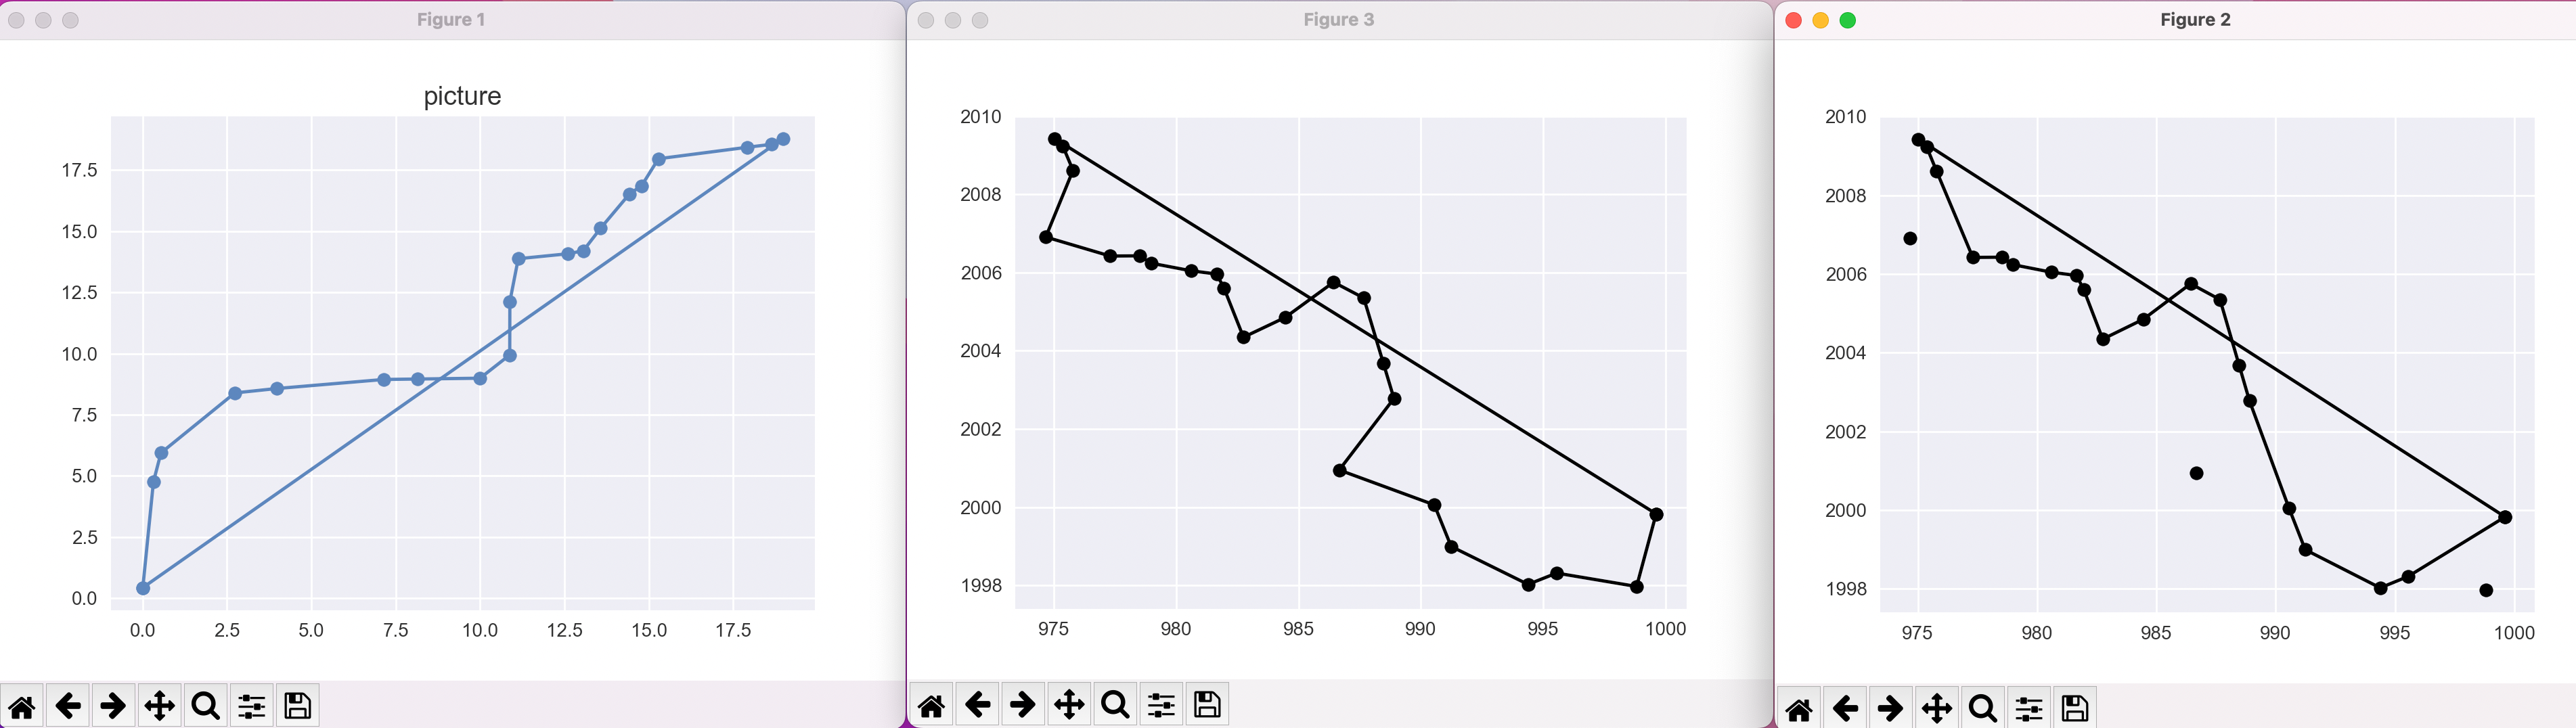
\includegraphics[width=0.9\textwidth]{2.png}
	\caption{\label{pr}Voting Tree Test}
	\end{figure}
This test data uses 23 points to match 20 points,The matched subgraph and the original graph are symmetrical to each other, and it can be seen from the results that the match is good.

\subsection*{Test2:}
You can see the test data in "data2.txt" and the match results in "output.txt"(I have submmit in my code).You can see the result next:
    \begin{figure}[H]
	\centering
	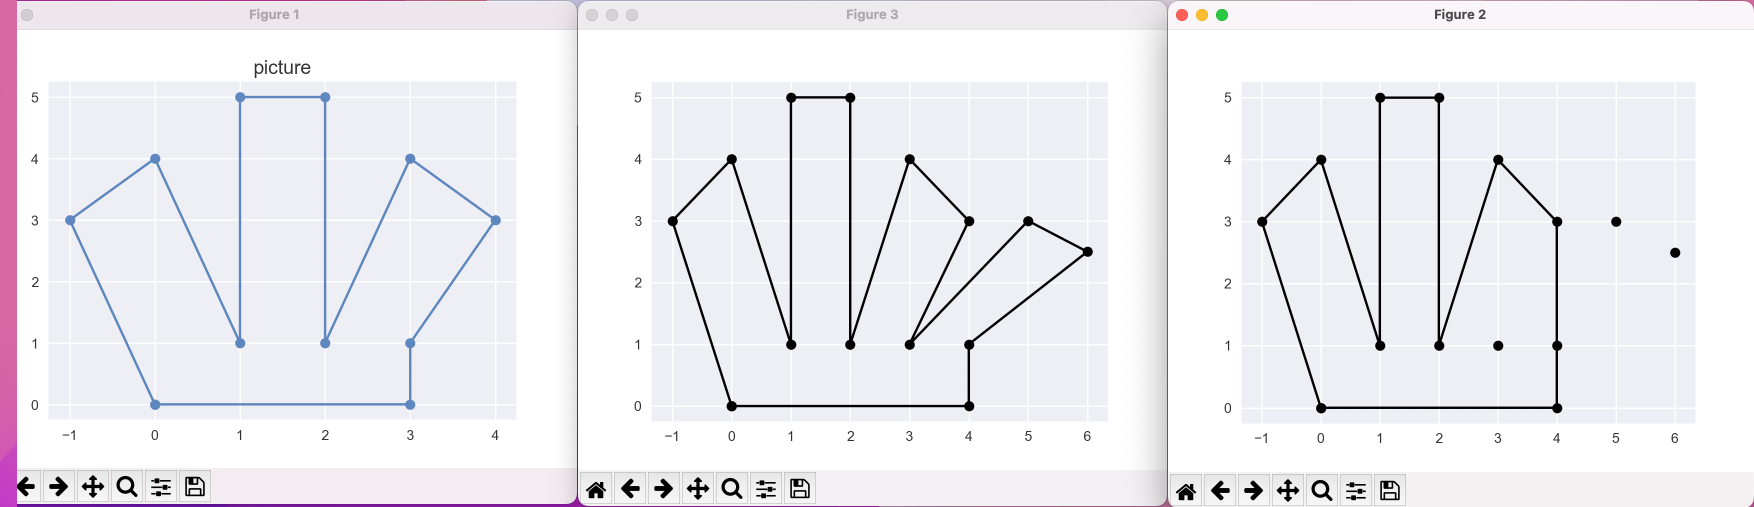
\includegraphics[width=0.9\textwidth]{3.png}
	\caption{\label{pr}Voting Tree Test}
	\end{figure}
This test data uses 14 points to match 11 points,There is no subgraph in the big graph that is exactly the same as the small graph, but the final match is still perfect

\subsection*{Test3:}
You can see the test data in "data3.txt" and the match results in "output.txt"(I have submmit in my code).You can see the result next:
    \begin{figure}[H]
	\centering
	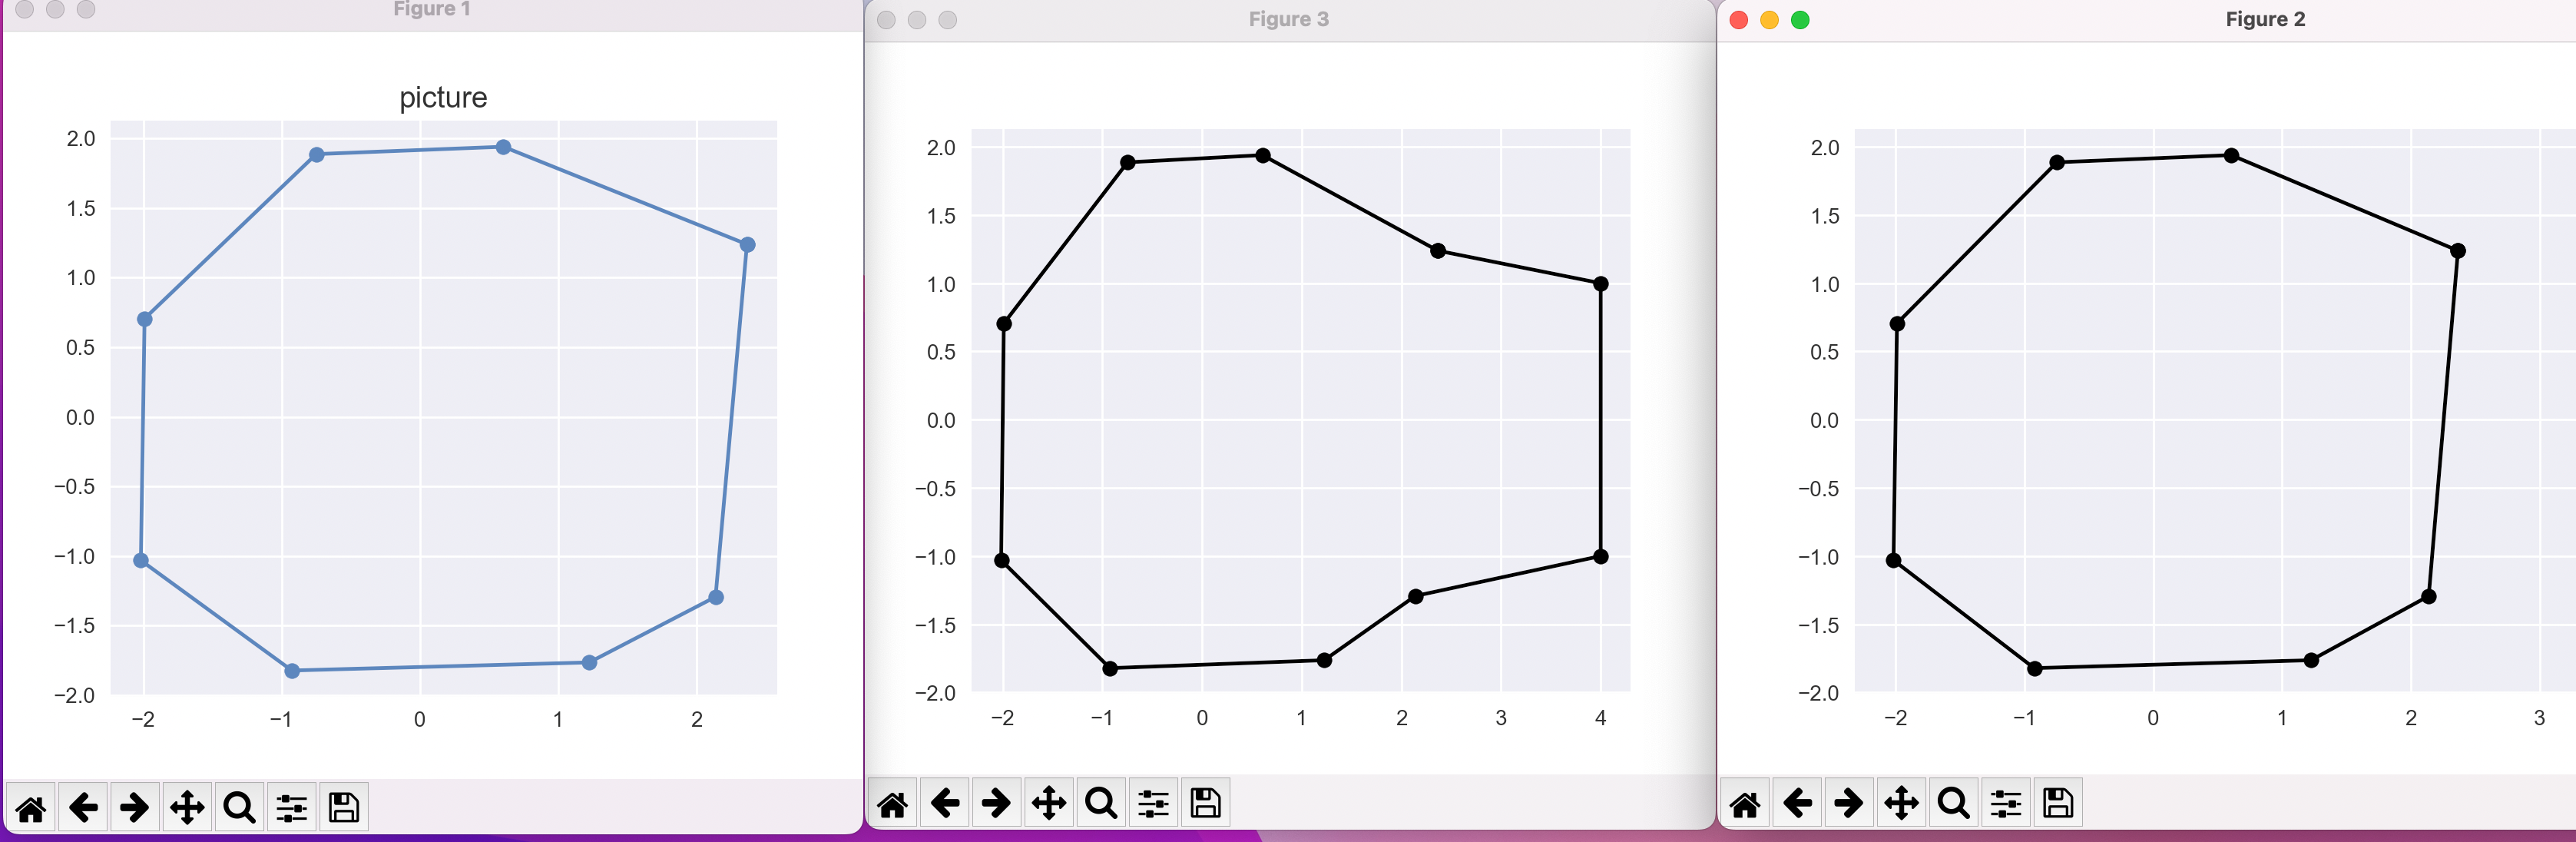
\includegraphics[width=0.9\textwidth]{4.png}
	\caption{\label{pr}Voting Tree Test}
	\end{figure}
This test data uses 10 points to match 8 points,the final match is still perfect

\subsection*{Test4:}
You can see the test data in "data4.txt" and the match results in "output.txt"(I have submmit in my code).You can see the result next:
    \begin{figure}[H]
	\centering
	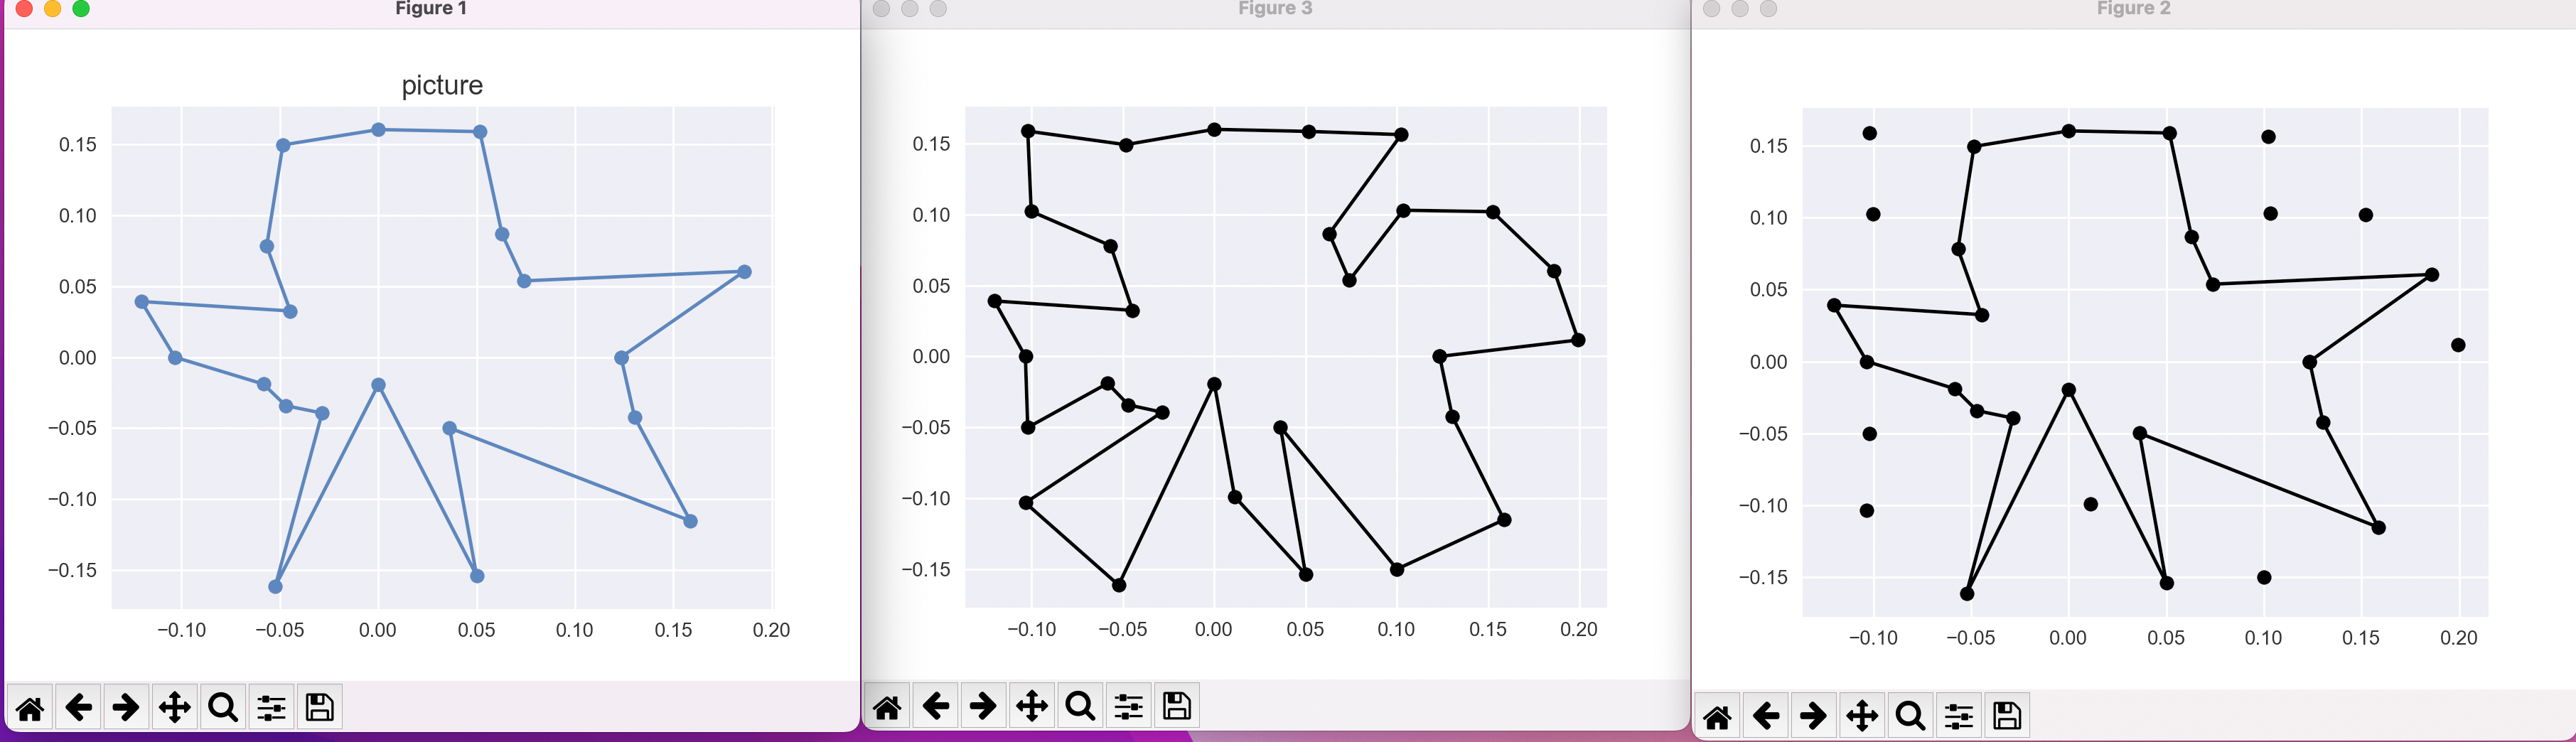
\includegraphics[width=0.9\textwidth]{5.png}
	\caption{\label{pr}Voting Tree Test}
	\end{figure}
This test data uses 30 points to match 20 points,the final match is still perfect.

\subsection*{Other Test:}
I still submmit some other test data and result in my code,if you are intersted in it,you can also test them.

\section*{Chaper 4:Analysis and Comments}
We suppose the less node number is M, the larger is N

\subsection*{Make a Tree:}

It starts from a root,to make a tree,the second level of this tree has (N-1) nodes,we will recursion expand it to totally M levels,
in each level we will use function Judge() to judge whether this nodes can be expanded or not,because of the limit of number of Nodes,
so there all actually $C_{N-1}^{M-1}$ ways can be used to make this tree in worst case.And by using the judge function,the complexities
will decrease a lot actually,and in each level the Node number can be expanded is O(N),so if we want to expanded a tree the time complexities 
is O(M*N) and when expanding a tree node we should new a location for it so its space complexity is also O(M*N).

\subsection*{Make a Forest:}
Because there are 2*N trees need to build so that the time complexities of Make this Forest is O(M*$N^{2}$) and its space complexities is O(M*$N^{2}$).

\subsection*{Delete Node:}
Use recursion to delete nodes that do not meet the path length requirements,its time complexity depends on the total number of paths,due to the limitation of passing conditions, there are not many complete paths that can be formed finally, which depends on the test data given.

\subsection*{Find the best match:}
If there are k roads totally,the time complexities of it is O(k).

\subsection*{possible boost:}
For the setting of the initial error threshold, I adopted the method of continuous trial and error from small to large to achieve the final judgment,It would be a nice boost to be able to quickly find a suitable margin of error.
But it can be seen from the test example that my method can still give a good judgment in the end, and it does not take long.If you have a good way, I hope you can give me some suggestions.
\section*{Appendix: Source Code (in C++)}



\section*{Declaration}
I hearby declare that all the work done in this project titled "Voting Tree" is of my independent effort.

\end{document}